\chapter{Deep Generative Modeling}\label{ch:overview-dgm}

\epigraph{
    \textit{What I cannot create, I do not understand.}}{Richard P. Feynman}

% \ys{This might be a good place to quote Richard Feynmann on ``What I cannot create, I do not understand.''}

% \jcc{need to rewrite the following: 
% At the heart of deep generative modeling (DGMs) is a compelling goal: teaching machines to create. Picture a system that studies thousands of images, musical pieces, or artworks—and then conjures something entirely new, yet strikingly faithful to the style and structure of its inspirations. This is more than copying; it is a learned capacity to generate original content grounded in the patterns of real-world data.}

% Deep generative models (DGMs) aim to approximate the complex and high dimensional probability distributions underlying real world data. Through unsupervised learning, they acquire the ability to synthesize novel artifacts such as images, text, video, or audio that are statistically consistent with the learned distribution.
% \se{this paragraph could be made more precise and clear}

Deep generative models (DGMs) are neural networks that learn a probability distribution over high-dimensional data (e.g., images, text, audio) so they can generate new examples that resemble the dataset. We denote the model distribution by $p_{\bphi}$ and the data distribution by $p_{\mathrm{data}}$. Given a finite dataset, we fit $\bphi$ by minimizing a loss that measures how far $p_{\bphi}$ is from $p_{\mathrm{data}}$. After training, generation amounts to running the model’s sampling procedure to draw $\rvx \sim p_{\bphi}$ (the density $p_{\bphi}(\rvx)$ may or may not be directly computable, depending on the model class). Model quality is judged by how well generated samples and their summary statistics match those of $p_{\mathrm{data}}$, together with task-specific or perceptual metrics.


This chapter builds the mathematical and conceptual foundations behind these ideas. We formalize the problem in \Cref{sec:formulation-dgm}, present representative model classes in \Cref{sec:examples-dgm}, and summarize a practical taxonomy in \Cref{sec:taxonomy}.

\chapterlearning{
  \item explain, in plain language, what a generative model is trying to learn from a dataset and what it means to model the data distribution;
  \item understand the core idea behind autoregressive models, VAEs, energy-based models, normalizing flows, GANs, and diffusion models, and see how they differ in the way they learn and generate new samples;
}{
If you are already familiar with the basic ideas behind modern generative models, you may skim this chapter and use it later as a quick reference.
}





% \ys{This type of motivating language is crucial to the success of the monograph, but it currently lacks the depth and force that a compelling vision should convey. I'd like to try rewriting all such paragraphs once we've addressed all the other issues.}
% \jcc{I rewrote it as the above brown part.}


% To understand how this creative synthesis becomes feasible, this chapter establishes the mathematical and conceptual foundations of modern generative models.

% We begin by formalizing the core problem in \Cref{sec:formulation-dgm}, introducing the key mathematical tools and notation that drive this field. While a diverse array of DGMs exists, as overviewed in \Cref{sec:examples-dgm}, our focus will narrow to three prominent classes of DGMs that are closely connected to diffusion models. These are: Variational Autoencoders (VAEs), which we discuss in \Cref{sec:vae}; Energy-Based Models (EBMs), introduced in \Cref{sec:ebm}; and Normalizing Flows (NFs), explored in \Cref{sec:flow-based-method}.  Through this exploration, readers will gain a comprehensive understanding of the principled foundations that underpin modern diffusion-based generative modeling, as developed in subsequent chapters.


\newpage
\section{What is Deep Generative Modeling?}\label{sec:formulation-dgm}

% \se{i feel a more algorithmic description describing the inputs (data) and the output (trained network) is the right level of abstraction to start}



DGMs take as input a large collection of real-world examples 
(e.g., images, text) drawn from an unknown and complex distribution $p_{\mathrm{data}}$ 
and output a trained neural network that parameterizes an approximate distribution $p_{\bphi}$. Their goals are twofold: 
\begin{enumerate}
\item \textbfs{Realistic Generation:} To generate novel, realistic samples indistinguishable from real data.
\item \textbfs{Controllable Generation:} To enable fine-grained and interpretable control over the generative process.
\end{enumerate}



% \ys{The words ``mimicry'' and ``mastery'' are unnecessarily obscure in this context.} \jcc{revised!}

% The capabilities of DGMs extend far beyond data synthesis. They have emerged as foundational tools across a wide range of domains: from restoring corrupted data and intelligently filling in missing information (inpainting) to simulating complex phenomena and driving new forms of creative content generation. \se{a bit odd to have this text here, isn't it contrallable generation?}

This section presents the fundamental concepts and motivations behind DGMs, preparing for a detailed exploration of their mathematical framework and practical applications.


\subsection{Mathematical Setup}\label{subsec:intro-math-setup}
Suppose we are given a finite collection of examples
$\{\rvx^{(i)}\}_{i=1}^N$, such as images, audio, or text.
We imagine that these examples were drawn from some underlying data distribution
$p_{\mathrm{data}}$, but we do not know this distribution explicitly.
In particular, we only observe the available training examples; we do not have a
formula for $p_{\mathrm{data}}$ or a direct procedure for drawing arbitrary new
samples from it\footnote{This is a common assumption in machine learning. For simplicity, we use the symbol $ p $ to represent either a probability distribution or its probability density/mass function, depending on the context.}.


\paragraph{Goal of DGM.}
The goal of deep generative modeling is therefore to learn a model that can
produce \emph{new} samples whose statistical characteristics resemble those of
the observed data.
We denote the distribution represented by a model with parameters
$\bm{\phi}$ by $p_{\bm{\phi}}$.
After training, we denote the learned parameters by $\bm{\phi}^{\times}$ and
hope that, in the aspects relevant to generation,
\[
    p_{\bm{\phi}^{\times}}
    \approx
    p_{\mathrm{data}}.
\]
This expression should be understood conceptually: with finite data, finite
model capacity, and imperfect optimization, we do not expect the two
distributions to be exactly identical.
Rather, the learned model should capture enough of the structure of the data
distribution to generate realistic and diverse new examples.

Once the model is trained, generation simply means drawing a new sample
\[
    \rvx \sim p_{\bm{\phi}^{\times}}.
\]
Different families of generative models provide different mechanisms for doing
this.
Some models additionally allow us to evaluate how much density they assign to
an observed sample, while others are primarily defined through their sampling
procedure.
This distinction will become useful later when we discuss how different
generative models are trained; for now, the central objective is simply to
learn a distribution from data from which we can generate new samples.
% The primary goal of DGM is to learn a tractable probability distribution from a finite dataset. These data points are observations assumed to be sampled from an unknown and complex true distribution $p_{\mathrm{data}}(\rvx)$. Since the form of $p_{\mathrm{data}}(\rvx)$ is unknown, we cannot draw new samples from it directly. The core challenge is therefore to create a model that approximates this distribution well enough to enable the generation of new, realistic samples.

% To this end, a DGM uses a deep neural network to parameterize a model distribution $p_{\bm{\phi}}(\rvx)$, where $\bm{\phi}$ represents the network's trainable parameters. The training objective is to find the optimal parameters $\bm{\phi}^\ast$ that minimize the divergence between the model distribution $p_{\bm{\phi}}(\rvx)$ and the true data distribution $p_{\mathrm{data}}(\rvx)$. Conceptually, 
% \[
% p_{{\bm{\phi}}^\ast}(\rvx) \approx p_{\mathrm{data}}(\rvx).
% \]




% The primary objective of deep generative modeling (DGM) is to learn \se{learn what?} from a finite dataset sampled from an unknown true distribution $p_{\mathrm{data}}(\mathbf{x})$, and to generate new samples that closely resemble this data. Since the explicit form of $p_{\mathrm{data}}(\mathbf{x})$ is unknown, the core challenge lies in approximating and efficiently sampling from this complex distribution \se{confusing, we never sample from pdata, only pmodel} to enable realistic and data-consistent generation based on limited observations.


% To this end, we use a deep neural network to construct a parametrized model density $p_{\bm{\phi}}(\rvx)$, where ${\bm{\phi}} \in \Phi$ denotes the model parameters \se{model and network terminology creates unnecessary ambiguity} and $\Phi$ represents the set of all possible parameter values. The objective is to find the optimal parameters ${\bm{\phi}}^\ast \in \Phi$ such that  
% \[
% p_{{\bm{\phi}}^\ast}(\rvx) \approx p_{\mathrm{data}}(\rvx).
% \]
% \se{i would rephrase slightly to avoid the potential confusion that networks have finite capacity so the above is not possible}

% When the statistical model $p_{{\bm{\phi}}^\ast}(\rvx)$ closely approximates the data distribution $p_{\mathrm{data}}(\rvx)$, it can serve as a proxy for generating new samples. This model $p_{\bm{\phi}}(\rvx)$ is commonly referred to as a \emph{generative model}.


% \paragraph{Capability of DGM.}
% Once a proxy of the data distribution, $p_{\bm{\phi}}(\rvx)$, is
% available, we can generate an arbitrary number of new data points using
% sampling methods such as Monte Carlo sampling from
% $p_{\bm{\phi}}(\rvx)$. Additionally, for any given sample $\rvx'$,
% we can evaluate the model density $p_{\bm{\phi}}(\rvx')$, which is
% often informally referred to as the model assigning a ``likelihood'' to
% $\rvx'$\footnote{For continuous data, $p_{\bm{\phi}}(\rvx')$ is
% strictly speaking the density evaluated at $\rvx'$, rather than the
% probability of observing that exact sample. We follow the common
% machine-learning shorthand of referring to this quantity as the sample's
% ``likelihood''.}.

\begin{figure}
\vspace{-0.5cm}
    \centering
    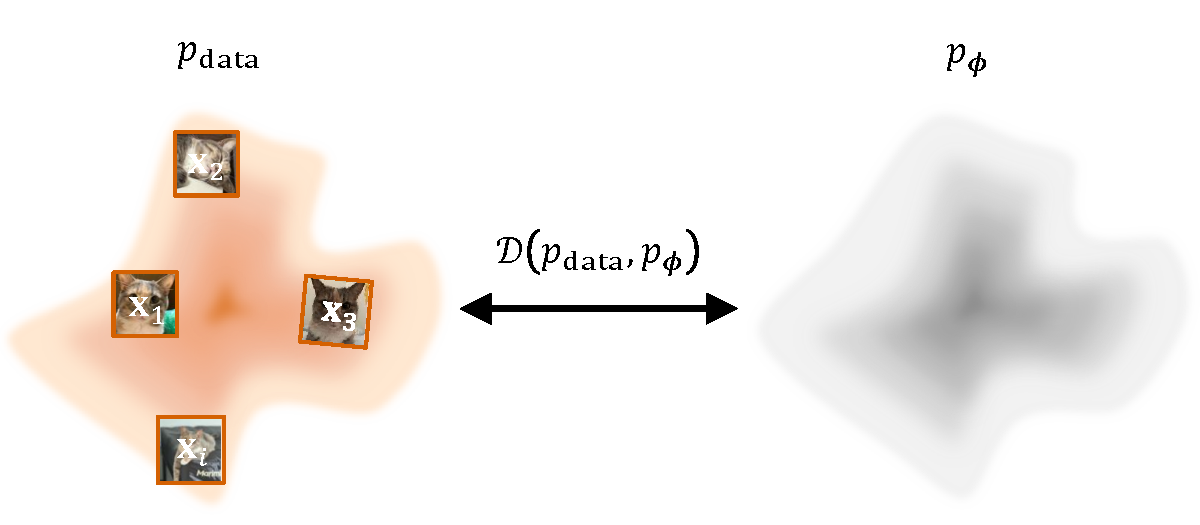
\includegraphics[width=0.9\linewidth]{Images/PartB/dgm-learning.pdf}
    \vspace{-0.2cm}
    \caption{\textbfs{Illustration of the target in DGM.} Training a DGM is essentially minimizing the discrepancy between the model distribution $p_{\bm{\phi}}$ and the unknown data distribution $p_{\mathrm{data}}$. Since $p_{\mathrm{data}}$ is not directly accessible, this discrepancy must be estimated efficiently using a finite set of independent and identically distributed (i.i.d.) samples, $\rvx_i$, drawn from it. \figcredit{Created by the authors.}}
    \label{fig:dgm-training}
\end{figure}

% \paragraph{Training of DGM.}
% To train the model, we define a discrepancy measure $\mathcal{D}(\cdot, \cdot)$ that quantifies the difference between the data distribution $p_{\mathrm{data}}$ and the model distribution $p_{\bm{\phi}}$. Since the true data distribution is unknown, this discrepancy must be estimated efficiently using a finite set of independent and identically distributed (i.i.d.) samples drawn from $p_{\mathrm{data}}$. The optimal parameter $\bm{\phi}^\ast$ is then obtained by solving the following optimization problem based on this empirical estimate:
% \begin{align}\label{eq:dgm-optimization}
%     \bm{\phi}^\ast = \arg\min_{\bm{\phi} \in \Phi} \mathcal{D}(p_{\mathrm{data}}, p_{\bm{\phi}}).
% \end{align}
% If the parameter space $\Phi$ is sufficiently large and the model family $\{p_{\bm{\phi}}\}_{\bm{\phi} \in \Phi}$ is expressive enough, then $p_{\bm{\phi}^\ast}(\mathbf{x})$ can closely approximate $p_{\mathrm{data}}(\mathbf{x})$.


% \ys{One missing factor is there must exist an efficient way to estimate this discrepancy measure using iid samples from the data distribution.}

% There are various choices for the discrepancy measure $\mathcal{D}$~\citep{cover1999elements}, including the Wasserstein distance, total variation distance, Jensen–Shannon divergence, Fisher divergence (spoiler: notably related to diffusion models), and the Kullback–Leibler (KL) divergence. Each induces a different training objective, with distinct trade-offs in sensitivity, smoothness, and optimization dynamics. Among them, the KL divergence is especially popular due to its close connection to maximum likelihood estimation, as discussed next.
% \se{instead of throwing all this jargon at the reader, i would start with an example (KL) and then tell them there are other options}

% \subparagraph{Kullback-Leibler Divergence.}
% \jc{
% A widely used choice for $\mathcal{D}$ is the Kullback–Leibler (KL) divergence, denoted by $\mathcal{D}_{\mathrm{KL}}(\cdot \| \cdot)$, which measures the discrepancy between the data distribution $p_{\mathrm{data}}$ and the model distribution $p_{\bm{\phi}}$. It is defined as
% \begin{align*}
%     \mathcal{D}_{\mathrm{KL}}(p_{\mathrm{data}} \| p_{\bm{\phi}}) 
%     &:= \int p_{\mathrm{data}}(\mathbf{x}) \log \frac{p_{\mathrm{data}}(\mathbf{x})}{p_{\bm{\phi}}(\mathbf{x})} \, \diff \mathbf{x} \\
%     &= \mathbb{E}_{p_{\mathrm{data}}} \left[ \log \frac{p_{\mathrm{data}}(\mathbf{x})}{p_{\bm{\phi}}(\mathbf{x})} \right],
% \end{align*}
% where the integral is a Lebesgue integral\footnote{Throuout the monograph, if without stating, the integration of deterministic mappings is understood as Lebesgue sense.}, which reduces to a summation when the distributions are defined over discrete spaces.

% The KL divergence is asymmetric, i.e., 
% \[
% \mathcal{D}_{\mathrm{KL}}(p_{\mathrm{data}} \| p_{\bm{\phi}}) \neq \mathcal{D}_{\mathrm{KL}}(p_{\bm{\phi}} \| p_{\mathrm{data}}).
% \]Importantly, minimizing $\mathcal{D}_{\mathrm{KL}}(p_{\mathrm{data}} \| p_{\bm{\phi}})$ encourages \emph{mode covering}: the model is penalized heavily if it assigns low probability to regions where the data density is high. This pushes the model to cover all modes of the data distribution, avoiding mode collapse.
% }
% \se{add an extra sentence actually showing it using the formula, e.g. if pmodel is zero when pdata is not}

% \ys{It may be useful to note somewhere that the integrals below refer to Lebesgue integrals, which reduce to summations when defined over counting measures.}

% \ys{No need to expand so much on the following list. Just mention it has the ``mode covering'' property, and explain what it means and why in a few sentences (ChatGPT can do this).} \jcc{Revised!}

% \se{important to note somewhere that pdata can't be evaluated, which is a good motivation for the MLE stuff below}

% Crucially, it is equivalent to \emph{Maximum Likelihood Estimation} (MLE), as detailed below.
% \subparagraph{Maximum Likelihood Training.}
% From the definition of $\mathcal{D}_{\mathrm{KL}}$, we derive:
% \begin{align*}
%     \mathcal{D}_{\mathrm{KL}}(p_{\mathrm{data}} \| p_{\bm{\phi}}) 
%     &= \displaystyle\int  \log \frac{p_{\mathrm{data}}(\mathbf{x})}{p_{\bm{\phi}}(\mathbf{x})} p_{\mathrm{data}}(\mathbf{x}) \diff \rvx \\
%     &= -\mathbb{E}_{\rvx \sim p_{\mathrm{data}}} \left[ \log p_{\bm{\phi}}(\mathbf{x}) \right] + C,
% \end{align*}
% where $C := \mathbb{E}_{\rvx \sim p_{\mathrm{data}}} \left[\log p_{\mathrm{data}}(\mathbf{x})\right]$ is constant with respect to $\bm{\phi}$. Hence, minimizing KL divergence is equivalent to maximizing the log-likelihood: 
% % \ys{``Message'' feels weird in this context. Maybe better to call it ``remark'', or ``observation''?}
% \msg{Observation}{Minimizing KL $\Leftrightarrow$ Maximum Likelihood Estimation}{
% \begin{align}\label{eq:MLE}
%     \min_{\bm{\phi}} \mathcal{D}_{\mathrm{KL}}(p_{\mathrm{data}} \| p_{\bm{\phi}}) \Longleftrightarrow \max_{\bm{\phi}}\mathbb{E}_{\rvx\sim p_{\mathrm{data}}}\left[\log p_{\bm{\phi}}(\rvx)\right].
% \end{align}
% }
% MLE is a classical method for learning probabilistic models by finding parameters $\bm{\phi}$ that maximize the likelihood of the observed data, rather than explicitly reconstructing the data points. \se{maybe move after you introduce the empirical (not population) version, otherwise there is no observation/data}

% To implement MLE in practice, we often minimize the KL divergence between the data and model distributions, approximated using a finite set of training samples  $\{\mathbf{x}^{(i)}\}_{i=1}^N$:
% \begin{align*}
%     \mathcal{D}_{\mathrm{KL}}(p_{\mathrm{data}} \| p_{\bm{\phi}}) 
%     &\approx  -\frac{1}{N} \sum_{i=1}^N \log p_{\bm{\phi}}(\mathbf{x}^{(i)}) + C,
% \end{align*}
% with $C = \frac{1}{N} \sum_{i=1}^N \log p_{\mathrm{data}}(\mathbf{x}^{(i)})$.
% \se{this is strange and potentially confusing, i would avoid the C estimate part since that is not something we can do "in practice"}


% \jc{While the model could theoretically assign arbitrarily high density to training points (a countable set with measure zero), in practice, neural networks avoid forming delta distributions due to their continuous and smooth architectures, finite capacity, and regularization (e.g., weight decay, dropout), which prevent overfitting.} \ys{I think you're confusing density functions with mass functions here. For continuous distributions, the optimal model distribution is indeed a delta distribution. The model's density function can take arbitrarily high values at data points, since these are countable. The integral of a probability density function is unaffected by its values on a countable set. The fact that our model distributions do not collapse to delta distributions cannot be attributed to the normalization constraint.} \jcc{Revised!}
% \se{not sure why overfitting/regularization is relevant here; it's not particularly specific to the loss used to train generative models}


\paragraph{Training of DGM.}
We learn parameters $\bm{\phi}$ of a model family $\{p_{\bm{\phi}}\}$ by minimizing a discrepancy $\mathcal{D}(p_{\mathrm{data}},p_{\bm{\phi}})$:
\begin{align}\label{eq:dgm-optimization}
  \bm{\phi}^\ast \in \arg\min_{\bm{\phi}}\; \mathcal{D}(p_{\mathrm{data}},p_{\bm{\phi}}).
\end{align}
Because $p_{\mathrm{data}}$ is unknown, a practical choice of $\mathcal{D}$ must admit efficient estimation from i.i.d.\ samples
from $ p_{\mathrm{data}}$. With sufficient capacity, $p_{\bm{\phi}^\ast}$ can closely approximate $p_{\mathrm{data}}$.

\subparagraph{Forward KL and Maximum Likelihood Estimation (MLE).}
How should we choose the model parameters so that
$p_{\bm{\phi}}$ resembles $p_{\mathrm{data}}$?
When the model density $p_{\bm{\phi}}(\rvx)$ can be evaluated, a natural idea is
to make the observed data receive high density under the model.
This leads to \emph{maximum likelihood estimation} (MLE): we choose
$\bm{\phi}$ so that the training examples are collectively assigned high model
density\footnote{For a fixed observed sample $\rvx$, the quantity
$p_{\bm{\phi}}(\rvx)$, viewed as a function of the model parameters
$\bm{\phi}$, is called the \emph{likelihood}. For continuous data,
$p_{\bm{\phi}}(\rvx)$ is a probability density rather than the probability of
observing exactly $\rvx$.}.

A standard way to formalize this idea is through the (forward)
Kullback--Leibler divergence\footnote{All integrals are in the Lebesgue sense
and reduce to sums under counting measures.}
\begin{align*}
\mathcal{D}_{\mathrm{KL}}
\big(p_{\mathrm{data}}\|p_{\bm{\phi}}\big)
:=\;&
\int
p_{\mathrm{data}}(\rvx)
\log
\frac{p_{\mathrm{data}}(\rvx)}
     {p_{\bm{\phi}}(\rvx)}
\,\diff \rvx
\\
=\;&
\mathbb{E}_{\rvx\sim p_{\mathrm{data}}}
\big[
\log p_{\mathrm{data}}(\rvx)
-
\log p_{\bm{\phi}}(\rvx)
\big].
\end{align*}
The KL divergence is asymmetric, i.e.,
\[
\mathcal{D}_{\mathrm{KL}}
\big(p_{\mathrm{data}}\|p_{\bm{\phi}}\big)
\neq
\mathcal{D}_{\mathrm{KL}}
\big(p_{\bm{\phi}}\|p_{\mathrm{data}}\big).
\]

At first, the forward KL may appear unusable because the data density
$p_{\mathrm{data}}(\rvx)$ is unknown.
However, it can be decomposed as
\begin{align*}
\mathcal{D}_{\mathrm{KL}}
\big(p_{\mathrm{data}}\|p_{\bm{\phi}}\big)
=
\mathbb{E}_{\rvx\sim p_{\mathrm{data}}}
\left[
\log
\frac{p_{\mathrm{data}}(\rvx)}
     {p_{\bm{\phi}}(\rvx)}
\right]
=
-\mathbb{E}_{\rvx\sim p_{\mathrm{data}}}
\big[
\log p_{\bm{\phi}}(\rvx)
\big]
-
\mathcal{H}\big(p_{\mathrm{data}}\big),
\end{align*}
where
\[
\mathcal{H}\big(p_{\mathrm{data}}\big)
:=
-\mathbb{E}_{\rvx\sim p_{\mathrm{data}}}
\big[
\log p_{\mathrm{data}}(\rvx)
\big]
\]
is the entropy of the data distribution.
Crucially, this term does not depend on $\bm{\phi}$.
Therefore, although we cannot evaluate $p_{\mathrm{data}}(\rvx)$ itself,
we do not need to know it in order to optimize the model parameters. This gives the following equivalence:
\lem{Minimizing KL $\Leftrightarrow$ MLE}{mle-kl}{
\begin{align}\label{eq:MLE}
\min_{\bm{\phi}}\,
\mathcal{D}_{\mathrm{KL}}
\big(
p_{\mathrm{data}}
\,\|\,
p_{\bm{\phi}}
\big)
\;\Longleftrightarrow\;
\max_{\bm{\phi}}\,
\mathbb{E}_{\rvx\sim p_{\mathrm{data}}}
\big[
\log p_{\bm{\phi}}(\rvx)
\big].
\end{align}
}

In words, minimizing the forward KL divergence is equivalent to making real
data samples receive high log-likelihood under the model.
This is exactly maximum likelihood estimation.

In practice, the expectation over $p_{\mathrm{data}}$ is replaced by the
available training samples
$\{\rvx^{(i)}\}_{i=1}^{N}$, assumed to be drawn i.i.d.\ from
$p_{\mathrm{data}}$.
This gives the empirical negative log-likelihood objective
\begin{align*}
\hat{\mathcal{L}}_{\mathrm{MLE}}(\bm{\phi})
:=
-\frac{1}{N}
\sum_{i=1}^{N}
\log p_{\bm{\phi}}\big(\rvx^{(i)}\big),
\end{align*}
which can be optimized using stochastic gradients over minibatches.
Thus, MLE requires only samples from $p_{\mathrm{data}}$; it does not require
evaluating the unknown data density itself.

The direction of the KL divergence matters because it determines
\emph{where the discrepancy is averaged}.
For the forward KL,
\[
\mathcal{D}_{\mathrm{KL}}
\big(p_{\mathrm{data}}\|p_{\bm{\phi}}\big)
=
\mathbb{E}_{\rvx\sim p_{\mathrm{data}}}
\left[
\log
\frac{p_{\mathrm{data}}(\rvx)}
     {p_{\bm{\phi}}(\rvx)}
\right],
\]
the expectation is taken over the data distribution.
Thus, regions that occur under $p_{\mathrm{data}}$ must be accounted for by
the model.
By contrast, the reverse KL,
$\mathcal{D}_{\mathrm{KL}}
(p_{\bm{\phi}}\|p_{\mathrm{data}})$,
averages instead over samples from the model distribution.

This difference has an important consequence.
Suppose there exists a region $A$ with positive data probability,
$p_{\mathrm{data}}(A)>0$, but the model assigns zero density there,
$p_{\bm{\phi}}(\rvx)=0$ for $\rvx\in A$.
Then the forward KL becomes infinite, since
\[
\log
\frac{p_{\mathrm{data}}(\rvx)}
     {p_{\bm{\phi}}(\rvx)}
=
+\infty
\]
on that region.
Therefore, minimizing the forward KL strongly penalizes a model for completely
missing regions where the data distribution places probability mass.
This behavior is commonly referred to as \emph{mode covering}.


\subparagraph{Fisher Divergence.} The Fisher divergence is another important concept for (score-based) diffusion modeling (see \Cref{ch:score-based}). For two distributions $p$ and $q$, it is defined as
\begin{align}\label{eq:fisher}
    \mathcal D_{\mathrm F}(p \|  q)
:=
\mathbb{E}_{\mathbf{x}\sim p} \left[
\left\|\nabla_{\mathbf x}\log p(\mathbf x)-\nabla_{\mathbf x}\log q(\mathbf x)\right\|_2^{2}
\right].
\end{align}
It measures the discrepancy between the \emph{score functions} 
$\nabla_{\mathbf x}\log p(\mathbf x)$ and $\nabla_{\mathbf x}\log q(\mathbf x)$,
which are vector fields pointing toward regions of higher probability. 
In short, $\mathcal D_{\mathrm F}(p \|  q)\ge 0$ with equality if and only if $p=q$ almost everywhere. 
It is invariant to normalization constants, since scores depend only on gradients of log-densities, 
and it forms the basis of \emph{score matching} (\Cref{eq:ebm-sm,eq:sm}): a method that learns the gradient of the log-density for generation (score-based models). 
In this setting, the data distribution $p=p_{\mathrm{data}}$ serves as the target, 
while the model $q=p_{\bm{\phi}}$ is trained to align its score field with that of the data.





\subparagraph{Beyond KL.} Although the KL divergence is the most widely used measure of difference between probability distributions, it is not the only one. Different divergences capture different geometric or statistical notions of discrepancy, which in turn affect the optimization dynamics of learning algorithms.  A broad family is the \emph{$f$-divergences}~\citep{csiszar1963informationstheoretische}:
\begin{align}\label{eq:f-div}
    \mathcal{D}_f(p\|q)
=\int q(\rvx) f \left(\frac{p(\rvx)}{q(\rvx)}\right)\diff \rvx,
\qquad f(1)=0,
\end{align}
where $f:\mathbb{R}_+ \to\mathbb{R}$ is a convex function.  
By changing $f$, we obtain many well-known divergences:
\[
\begin{aligned}
f(u)&=u\log u &&\Rightarrow&& \mathcal{D}_f=\mathcal{D}_{\mathrm{KL}}(p\|q)\quad\text{(forward KL)},\\
f(u)&=\tfrac12 \left[u\log u-(u+1)\log \tfrac{1+u}{2}\right] &&\Rightarrow&& \mathcal{D}_f=\mathcal{D}_{\mathrm{JS}}(p\|q)\quad\text{(Jensen--Shannon)},\\
f(u)&=\tfrac12|u-1| &&\Rightarrow&& \mathcal{D}_f=\mathcal{D}_{\mathrm{TV}}(p,q)\quad\text{(total variation)}.
\end{aligned}
\]
For clarity, the explicit forms are
\[
\mathcal{D}_{\mathrm{JS}}(p\|q)=\tfrac12 \mathcal{D}_{\mathrm{KL}}\big(p\| \tfrac12(p+q)\big)+\tfrac12 \mathcal{D}_{\mathrm{KL}}\big(q\| \tfrac12(p+q)\big),
\]
and
\[
\mathcal{D}_{\mathrm{TV}}(p,q)=\tfrac12 \int_{\mathbb{R}^D
} |p-q|\diff \rvx
=\sup_{A\subset \mathbb{R}^D } |p(A)-q(A)|.
\]
Intuitively, the JS divergence provides a smooth and symmetric measure that balances both distributions and avoids the unbounded penalties of KL (we will later see that it helps interpret the Generative Adversarial Network (GAN) framework), while the total variation distance captures the largest possible probability difference between the two.


A different viewpoint comes from \emph{optimal transport} (see \Cref{ch:ot-eot}), whose representative is the Wasserstein distance (see \Cref{eq: Monge's Formulation}). It measures the minimal cost of moving probability mass from one distribution to another. Unlike $f$-divergences, which compare density ratios, Wasserstein distances depend on the geometry of the sample space and remain meaningful even when the supports of $p$ and $q$ do not overlap.

Each divergence embodies a different notion of closeness between distributions and thus induces distinct learning behavior. We will revisit these divergences when they arise naturally in the context of generative modeling throughout this monograph.







\subsection{Challenges in Modeling Distributions}
% We recall that a valid probability density function $p(\rvx)$ must satisfy the following conditions:
% \begin{enumerate}\label{eq:pdf-cond}
%     \item[(i)] \textbfs{Non-Negativity:} 
%     \[
%     p(\rvx) \geq 0, \quad \text{for all } \rvx \in \mathbb{R}^D;
%     \]
%     \item[(ii)] \textbfs{Normalization:} 
%     \[
%     \int p(\rvx) \diff \rvx = 1.
%     \]
% \end{enumerate}

% When modeling $p_{\mathrm{data}}$ with a neural network $E_{\bm{\phi}}\colon\mathbb{R}^D\rightarrow\mathbb R$, both conditions must be satisfied. 
% \se{this change of notation (from pphi to Ephi) is confusing}
% Enforcing (i) is straightforward: common transformations such as
% \[
% e^{-E_{\bm{\phi}}(\rvx)}, \quad \abs{E_{\bm{\phi}}(\rvx)}, \quad E^2_{\bm{\phi}}(\rvx), \quad \text{etc.}
% \]
% can ensure non-negativity. To enforce (ii), we normalize the output:
% \[
%  \frac{E_{\bm{\phi}}(\rvx)}{\int E_{\bm{\phi}}(\rvx) \diff \rvx}, 
% \]
% where $Z({\bm{\phi}}):=\int E_{\bm{\phi}}(\rvx) \diff \rvx$ is the normalizing constant. However, computing $Z({\bm{\phi}})$ is often intractable due to the high-dimensional integral over the data space.

% \se{i think this section needs a bit more guidance, starting from how one might use a neural net to represent the density/pmf scalar function, and the constraints needed}



% \newpage
To model a complex data distribution, we can parameterize the probability density function $p_{\mathrm{data}}$ using a neural network with parameters $\bm{\phi}$, creating a model we denote as $p_{\bm{\phi}}$. For $p_{\bm{\phi}}$ to be a valid probability density function, it must satisfy two fundamental properties:
\begin{enumerate}
    \item[(i)] \textbfs{Non-Negativity:} $p_{\bm{\phi}}(\rvx) \ge 0$ for all $\rvx$ in the domain.
    \item[(ii)] \textbfs{Normalization:} The integral over the entire domain must equal one, i.e., $\int p_{\bm{\phi}}(\rvx) \diff \rvx = 1$.
\end{enumerate}

A network can naturally produce a real scalar $E_{\bphi}(\rvx) \in \R$ for input $\rvx$. To interpret this output as a valid density, it must be transformed to satisfy conditions (i) and (ii).  
A practical alternative is to view $E_{\bphi}\colon\mathbb{R}^D\to\mathbb{R}$ as defining an \emph{unnormalized} density and then enforce these properties explicitly.


\paragraph{Step 1: Ensuring Non-Negativity.}
We can guarantee that our model's output is always non-negative by applying a positive function to the raw output of the neural network $E_{\bm{\phi}}(\rvx)$, such as $\abs{E_{\bm{\phi}}(\rvx)}$, $E^2_{\bm{\phi}}(\rvx)$. A standard and convenient choice is the exponential function. This gives us an unnormalized density, $\tilde{p}_{\bm{\phi}}(\rvx)$, that is guaranteed to be positive:
\[
\tilde{p}_{\bm{\phi}}(\rvx) = \exp(E_{\bm{\phi}}(\rvx)).
\]

\paragraph{Step 2: Enforcing Normalization.}
The function $\tilde{p}_{\bm{\phi}}(\rvx)$ is positive but does not integrate to one. To create a valid probability density, we must divide it by its integral over the entire space. This leads to the final form of our model:
\[
p_{\bm{\phi}}(\rvx) = \frac{\tilde{p}_{\bm{\phi}}(\rvx)}{\int \tilde{p}_{\bm{\phi}}(\rvx') \diff \rvx'} = \frac{\exp(E_{\bm{\phi}}(\rvx))}{\int \exp(E_{\bm{\phi}}(\rvx')) \diff \rvx'}.
\]
The denominator in this expression is known as the \emph{normalizing constant} or \emph{partition function}, denoted by $Z(\bm{\phi})$:
\[
Z(\bm{\phi}) := \int \exp(E_{\bm{\phi}}(\rvx')) \diff \rvx'.
\]
While this procedure provides a valid construction for $p_{\bm{\phi}}(\rvx)$, it introduces a major computational challenge. For most high-dimensional problems, the integral required to compute the normalizing constant $Z(\bm{\phi})$ is intractable. This intractability is a central problem that motivates the development of many different families of deep generative models.


In the following sections, we introduce several prominent approaches of DGM. Each is designed to circumvent or reduce the computational cost of evaluating this normalizing constant.
\newpage



\begin{figure}[th!]
\centering
\resizebox{\linewidth}{!}{%
\begin{tikzpicture}[
  ->, >=Stealth, thick, font=\normalsize,
  x=2.6cm, y=2.0cm,
  every node/.style={outer sep=0pt}
]
% ============= Styles (single source of truth) =============
\tikzset{
  state/.style={
    rectangle, rounded corners=3pt,
    draw=black, fill=gray!10,
    minimum height=10mm, minimum width=14mm, % same for all variables
    align=center, inner sep=2pt,
    font=\Large % <-- enlarge text in ALL variable nodes (x, x', x_t, z, ...)
  },
  stategap/.style={ % invisible box with SAME size as state, for equal arrow lengths
    rectangle, rounded corners=3pt,
    draw=none, fill=none,
    minimum height=10mm, minimum width=14mm,
    align=center, inner sep=2pt
  },
  processor/.style={
    trapezium, trapezium stretches=true,
    trapezium left angle=80, trapezium right angle=80,
    draw=black, fill=gray!20,
    minimum height=12mm, minimum width=28mm, align=center, inner sep=2pt
  },
  ovalval/.style={
    draw, ellipse, fill=gray!10,
    minimum height=7mm, minimum width=20mm, align=center
  },
  flowblock/.style={ % NF function blocks
    rectangle, rounded corners=3pt,
    draw=black, fill=gray!20,
    minimum height=12mm, minimum width=28mm, align=center, inner sep=3pt
  }
}

% ============= Shared column anchors (perfect row alignment) =============
\coordinate (L) at (0,0);    % left column
\coordinate (M) at (2.0,0);  % (kept for reference)
\coordinate (R) at (4.8,0);  % right column
\coordinate (C) at ($ (L)!0.5!(R) $); % true midpoint between L and R

% Vertical offsets for rows
\def\rowA{0}       % Row 1: EBM
\def\rowB{-1.3}    % Row 2: AR
\def\rowC{-3.0}    % Row 3: VAE
\def\rowD{-4.7}    % Row 4: NF
\def\rowE{-7.1}    % Row 5: GAN (two floors)
\def\rowF{-8.5}    % Row 6: DM

% Row tags
\node[anchor=east] at ($(L)+(-0.5,\rowA)$) {\textbfs{EBM}};
\node[anchor=east] at ($(L)+(-0.5,\rowB)$) {\textbfs{AR}};
\node[anchor=east] at ($(L)+(-0.5,\rowC)$) {\textbfs{VAE}};
\node[anchor=east] at ($(L)+(-0.5,\rowD)$) {\textbfs{NF}};
\node[anchor=east] at ($(L)+(-0.5,\rowE)$) {\textbfs{GAN}};
\node[anchor=east] at ($(L)+(-0.5,\rowF)$) {\textbfs{DM}};

% ====================== Row 1: EBM (unchanged) ======================
\node[state]   (ebm-x)   at ($(L)+(0,\rowA)$) {$\rvx$};
\node[ovalval] (ebm-val) at ($(C)+(0,\rowA)$) {value};
\coordinate (midE) at ($ (ebm-x.east)!0.5!(ebm-val.west) $);
\node[processor, shape border rotate=270] (ebm-energy) at (midE)
  {\footnotesize\textbfs{Energy}\\[-2pt]\footnotesize $E_{\bm\phi}(\rvx)$};
\draw (ebm-x.east) -- (ebm-energy.west);
\draw (ebm-energy.east) -- (ebm-val.west);

% ====================== Row 2: AR (unchanged) =======================
\coordinate (Lb) at ($(L)+(0,\rowB)$);
\coordinate (Rb) at ($(R)+(0,\rowB)$);
\node[state]   (ar-x)    at ($ (Lb)!0/6!(Rb) $) {$\rvx_0$};
\node[state]   (ar-x0)   at ($ (Lb)!1/6!(Rb) $) {$\rvx_{1}$};
\node[state]   (ar-x1)   at ($ (Lb)!2/6!(Rb) $) {$\rvx_{2}$};
\node[state]   (ar-x2)   at ($ (Lb)!3/6!(Rb) $) {$\rvx_{3}$}; % centered at C
\node[stategap](ar-gap)  at ($ (Lb)!4/6!(Rb) $) {};
\node[state]   (ar-xLm1) at ($ (Lb)!5/6!(Rb) $) {$\rvx_{L-1}$};
\node[state]   (ar-xL)   at ($ (Lb)!6/6!(Rb) $) {$\rvx_{L}$};
\node at (ar-gap) {$\boldsymbol{\cdots}$};
\draw (ar-x.east)    -- (ar-x0.west);
\draw (ar-x0.east)   -- (ar-x1.west);
\draw (ar-x1.east)   -- (ar-x2.west);
\draw (ar-x2.east)   -- (ar-gap.west);
\draw (ar-gap.east)  -- (ar-xLm1.west);
\draw (ar-xLm1.east) -- (ar-xL.west);
% Optional arcs
\draw (ar-x.south)    to[out=-35, in=-145] (ar-x2.south);
\draw (ar-x0.south)   to[out=-40, in=-140] (ar-x2.south);
\draw (ar-gap.south)  to[out=-40, in=-140] (ar-xL.south);
\draw (ar-xLm1.south) to[out=-55, in=-125] (ar-xL.south);

% ====================== Row 3: VAE (unchanged) =======================
\node[state] (vae-x)   at ($(L)+(0,\rowC)$) {$\rvx$};
\node[state] (vae-z)   at ($(C)+(0,\rowC)$) {$\rvz$};
\node[state] (vae-xp)  at ($(R)+(0,\rowC)$) {$\rvx'$};
\coordinate (midEnc) at ($ (vae-x.east)!0.5!(vae-z.west) $);
\node[processor, shape border rotate=270] (vae-enc) at (midEnc)
  {\footnotesize\textbfs{Encoder}\\[-2pt]\footnotesize $q_{\bm\theta}(\rvz|\rvx)$};
\coordinate (midDec) at ($ (vae-z.east)!0.5!(vae-xp.west) $);
\node[processor, shape border rotate=90] (vae-dec) at (midDec)
  {\footnotesize\textbfs{Decoder}\\[-2pt]\footnotesize $p_{\bm\phi}(\rvx|\rvz)$};
\draw (vae-x.east)   -- (vae-enc.west);
\draw (vae-enc.east) -- (vae-z.west);
\draw (vae-z.east)   -- (vae-dec.west);
\draw (vae-dec.east) -- (vae-xp.west);

% ====================== Row 4: NF (unchanged) =======================
\node[state] (nf-x)  at ($(L)+(0,\rowD)$) {$\rvx$};
\node[state] (nf-z)  at ($(C)+(0,\rowD)$) {$\rvz$};
\node[state] (nf-xp) at ($(R)+(0,\rowD)$) {$\rvx'$};
\coordinate (midFwd) at ($ (nf-x.east)!0.5!(nf-z.west) $);
\coordinate (midInv) at ($ (nf-z.east)!0.5!(nf-xp.west) $);
\node[flowblock] (nf-forward) at (midFwd)
  {\footnotesize\textbfs{Forward}\\[-1pt]\footnotesize $\rvf_{\bm\phi}(\rvx)$};
\node[flowblock] (nf-inverse) at (midInv)
  {\footnotesize\textbfs{Inverse}\\[-1pt]\footnotesize $\rvf_{\bm\phi}^{-1}(\rvz)$};
\draw (nf-x.east)       -- (nf-forward.west);
\draw (nf-forward.east) -- (nf-z.west);
\draw (nf-z.east)       -- (nf-inverse.west);
\draw (nf-inverse.east) -- (nf-xp.west);

% ====================== Row 5: GAN (two floors; unchanged) =======================
\def\gansep{0.9} % vertical gap between lower and upper floors
\node[state] (gan-z)  at ($(L)+(0,\rowE)$) {$\rvz$};
\node[state] (gan-xp) at ($(C)+(0,\rowE)$) {$\rvx'$};
\coordinate (midGen) at ($ (gan-z.east)!0.5!(gan-xp.west) $);
\node[processor, shape border rotate=90] (gan-gen) at (midGen)
  {\footnotesize\textbfs{Generator}\\[-2pt]\footnotesize $\rmG_{\bm\phi}(\rvz)$};
\node[state]   (gan-x)   at ($(C)+(0,\rowE+\gansep)$) {$\rvx$};
\node[ovalval] (gan-val) at ($(R)+(0,\rowE+\gansep)$) { 0/1};
\coordinate (midDisc) at ($ (gan-x.east)!0.5!(gan-val.west) $);
\node[processor, shape border rotate=270] (gan-disc) at (midDisc)
  {\footnotesize\textbfs{Discriminator}\\[-2pt]\footnotesize $D_{\bm\zeta}$};
\draw (gan-z.east)   -- (gan-gen.west);
\draw (gan-gen.east) -- (gan-xp.west);
\draw (gan-x.east)   -- (gan-disc.west);
\draw (gan-xp.east)  -- (gan-disc);
\draw (gan-disc.east) -- (gan-val.west);

% ====================== Row 6: DM (aligned with AR; equal-length arrows) =======================
% Use the same 7 centers as AR, anchored at L and R
\coordinate (Lf) at ($(L)+(0,\rowF)$);
\coordinate (Rf) at ($(R)+(0,\rowF)$);

\node[state]    (dm-x)     at ($ (Lf)!0/6!(Rf) $) {$\rvx_0$};
\node[state]    (dm-x0)    at ($ (Lf)!1/6!(Rf) $) {$\rvx_{1}$};
\node[state]    (dm-x1)    at ($ (Lf)!2/6!(Rf) $) {$\rvx_{2}$};
\node[state]    (dm-x2)    at ($ (Lf)!3/6!(Rf) $) {$\rvx_{3}$}; % exactly the same x as AR's x_2 and C
\node[stategap] (dm-gap)   at ($ (Lf)!4/6!(Rf) $) {};
\node[state]    (dm-xLm1)  at ($ (Lf)!5/6!(Rf) $) {$\rvx_{L-1}$};
\node[state]    (dm-xL)    at ($ (Lf)!6/6!(Rf) $) {$\rvx_{L}$};

% Draw the dots on top of the invisible gap box (no effect on spacing)
\node at (dm-gap) {$\boldsymbol{\cdots}$};

% Offsets for top (dashed) and bottom (solid) channels
\def\dmshift{4.5pt}

% Forward noising (top dashed; equal visible lengths)
\draw[dashed] ([yshift=\dmshift]dm-x.east)     -- ([yshift=\dmshift]dm-x0.west);
\draw[dashed] ([yshift=\dmshift]dm-x0.east)    -- ([yshift=\dmshift]dm-x1.west);
\draw[dashed] ([yshift=\dmshift]dm-x1.east)    -- ([yshift=\dmshift]dm-x2.west);
\draw[dashed] ([yshift=\dmshift]dm-x2.east)    -- ([yshift=\dmshift]dm-gap.west);
\draw[dashed] ([yshift=\dmshift]dm-gap.east)   -- ([yshift=\dmshift]dm-xLm1.west);
\draw[dashed] ([yshift=\dmshift]dm-xLm1.east)  -- ([yshift=\dmshift]dm-xL.west);

% Reverse denoising (bottom solid; equal visible lengths)
\draw ([yshift=-\dmshift]dm-x0.west)  -- ([yshift=-\dmshift]dm-x.east);
\draw ([yshift=-\dmshift]dm-x1.west)  -- ([yshift=-\dmshift]dm-x0.east);
\draw ([yshift=-\dmshift]dm-x2.west)  -- ([yshift=-\dmshift]dm-x1.east);
\draw ([yshift=-\dmshift]dm-gap.west) -- ([yshift=-\dmshift]dm-x2.east);
\draw ([yshift=-\dmshift]dm-xLm1.west)-- ([yshift=-\dmshift]dm-gap.east);
\draw ([yshift=-\dmshift]dm-xL.west)  -- ([yshift=-\dmshift]dm-xLm1.east);

\end{tikzpicture}}%
\vspace{1.0cm}
\caption{\textbfs{Computation graphs of prominent deep generative models.} Top to bottom: \textbfs{EBM} maps an input $\rvx$ to a scalar energy; \textbfs{AR} generates a sequence $\{\rvx_\ell\}_{\ell=0}^{L}$ left to right with causal dependencies; \textbfs{VAE} encodes $\rvx$ to a latent $\rvz$ and decodes to a reconstruction $\rvx'$; \textbfs{NF} applies an invertible map $\rvf_\bphi$ between $\rvx$ and $\rvz$ and uses $\rvf_\bphi^{-1}$ to produce $\rvx'$; \textbfs{GAN} transforms noise $\rvz$ to a sample $\rvx'$ that is judged against real $\rvx$ by a discriminator $D_{\bm\zeta}$; \textbfs{DM} iteratively refines a noisy sample through a multi-step denoising chain $\{\rvx_\ell\}_{\ell=0}^{L}$. Boxes denote variables, trapezoids are learnable networks, ovals are scalars; arrows indicate computation flow. The trapezoid was intended to indicate a dimension-changing transformation, while rectangles denote variables or mappings that preserve dimensionality. \figcredit{Created by the authors.}}
\label{fig:ebm-ar-vae-nf-gan-dm-unified}
\end{figure}
\newpage

\section{Prominent Deep Generative Models}\label{sec:examples-dgm}





A central challenge in generative modeling is to learn expressive probabilistic models that can capture the rich and complex structure of high-dimensional data. Over the years, various modeling strategies have been developed, each making different trade-offs between tractability, expressiveness, and training efficiency. In this section, we explore some of the most influential strategies that have
shaped the field, accompanied by a comparison of their computation graphs in
\Cref{fig:ebm-ar-vae-nf-gan-dm-unified}.



% \ys{Avoid using fancy words. It’s not that you can’t use “advanced” terms like tapestry, but these words are rare for a reason: they’re hard to use well and should only appear when truly appropriate, which isn’t the case here.}

% \se{why this order? i would start with the easiest, so either AR or EBM}

% \se{this VAE paragraph is full of undefined jargon and will make little to no sense to a non-expert reader}



\paragraph{Energy-Based Models (EBMs).}
EBMs~\citep{ackley1985learning,lecun2006tutorial} define a probability distribution through an energy function $ E_{\bm{\phi}}(\rvx) $ that assigns lower energy to more probable data points. The probability of a data point is defined as:
\begin{equation*}
    p_{\bm{\phi}}(\rvx) := \frac{1}{Z({\bm{\phi}})} \exp(-E_{\bm{\phi}}(\rvx)),
\end{equation*}
where 
\[Z({\bm{\phi}}) = \int \exp(-E_{\bm{\phi}}(\rvx)) \diff\rvx\] 
is the partition function. Training EBMs typically involves maximizing the log-likelihood of the data. However, this requires techniques to address the computational challenges arising from the intractability of the partition function. In the following chapter, we will explore how Diffusion Models offer an alternative by generating data from \emph{the gradient of the log density}, which does not depend on the normalizing constant, thereby circumventing the need for partition function computation.


% \begin{figure}[tbh!]
% \centering
% \resizebox{0.6\linewidth}{!}{%
% \begin{tikzpicture}[>=Latex, thick, font=\normalsize, node distance=0.8cm]

% \tikzset{
%   state/.style={
%     rectangle, rounded corners=3pt,
%     draw=black, fill=gray!10,
%     minimum height=28pt, minimum width=18pt, align=center,
%     outer sep=0pt, inner sep=2pt
%   },
%   encoderblock/.style={
%     trapezium, trapezium stretches=true,
%     trapezium left angle=80, trapezium right angle=80,
%     shape border rotate=270,
%     draw=black, fill=gray!20,
%     minimum height=6pt, minimum width=12pt, inner sep=2pt, align=center
%   },
%   decoderblock/.style={
%     trapezium, trapezium stretches=true,
%     trapezium left angle=80, trapezium right angle=80,
%     shape border rotate=90,
%     draw=black, fill=gray!20,
%     minimum height=6pt, minimum width=12pt, inner sep=2pt, align=center
%   }
% }

% % --- EBM nodes (smaller) ---
% \node[state] (x) {$\mathbf{x}$};
% \node[decoderblock, right=of x, minimum height=34pt, minimum width=56pt, inner sep=2pt] (energy)
%   {\footnotesize\textbfs{Energy Function}\\[-3pt]\footnotesize $E_{\bm{\phi}}(\mathbf{x})$};
% \node[draw, ellipse, fill=gray!10, right=of energy,
%       minimum height=16pt, minimum width=32pt, align=center, inner sep=1.5pt] (val)
%   {\footnotesize value};

% % arrows
% \draw[->] (x) -- (energy);
% \draw[->] (energy) -- (val);

% \end{tikzpicture}}
% \caption{\textbfs{Energy-based model (EBM).} The energy function $E_{\bm{\phi}}(\mathbf{x})$ maps an input $\mathbf{x}$ to a scalar energy; lower energy implies higher likelihood $p_{\bm{\phi}}(\mathbf{x}) \propto \exp \big(-E_{\bm{\phi}}(\mathbf{x})\big)$.}
% \label{fig:ebm-graph}
% \end{figure}



\paragraph{Autoregressive Models.}
Deep autoregressive (AR) models~\citep{frey1995does,larochelle2011neural,uria2016neural}
build on a simple but powerful observation: any joint distribution can be decomposed into a sequence of conditional distributions using the \emph{chain rule of probability}. 
For a chosen ordering of the variables $\mathbf{x}=(x_1,\ldots,x_D)$, the data distribution satisfies
\begin{equation*}
    p_{\mathrm{data}}(\mathbf{x})
    =
    \prod_{i=1}^{D}
    p_{\mathrm{data}}(x_i | \mathbf{x}_{<i}),
    \qquad
    \mathbf{x}_{<i}=(x_1,\ldots,x_{i-1}).
\end{equation*}
Importantly, this factorization is an exact identity rather than a modeling assumption: any joint distribution admits such a decomposition for any chosen ordering of its variables.

The challenge is that the true conditional distributions
$p_{\mathrm{data}}(x_i|\mathbf{x}_{<i})$ are unknown.
AR models therefore parameterize a model with the same factorized form,
\begin{equation*}
    p_{\bm{\phi}}(\mathbf{x})
    =
    \prod_{i=1}^{D}
    p_{\bm{\phi}}(x_i|\mathbf{x}_{<i}),
\end{equation*}
and use a neural network, such as a Transformer, to approximate these conditional distributions from data.
For example, for discrete data the network may output a categorical distribution through a softmax, whereas for continuous data it may output the parameters of a tractable conditional density.
Because every conditional distribution is normalized, their product automatically defines a normalized joint distribution.

This construction also makes likelihood-based training particularly simple.
For a data sample $\mathbf{x}$, the log-likelihood decomposes as
\begin{equation*}
    \log p_{\bm{\phi}}(\mathbf{x})
    =
    \sum_{i=1}^{D}
    \log p_{\bm{\phi}}(x_i|\mathbf{x}_{<i}),
\end{equation*}
so the model can be trained directly by maximum likelihood, or equivalently by minimizing the negative log-likelihood.
During training, the observed preceding variables $\mathbf{x}_{<i}$ are available, so many of these conditional predictions can typically be evaluated in parallel.

Generation, however, remains inherently sequential:
\begin{equation*}
    x_1 \sim p_{\bm{\phi}}(x_1),
    \qquad
    x_2 \sim p_{\bm{\phi}}(x_2| x_1),
    \qquad
    \ldots,
    \qquad
    x_D \sim p_{\bm{\phi}}(x_D|\mathbf{x}_{<D}).
\end{equation*}
Thus, AR models provide tractable exact likelihoods and flexible density modeling, but sampling requires generating variables one after another and can therefore become computationally expensive for long sequences. AR models remain a foundational class of likelihood-based generative models and underlie many modern sequence and language models.

% \begin{figure}[tbh!]
%     \centering
%     \resizebox{\linewidth}{!}{%
% \begin{tikzpicture}[
%     ->, >=Stealth, thick,
%     node_dist/.style={right=1.7cm of #1},
%     font=\small
%   ]

%   % Node style
%   \tikzset{state/.style={
%       rectangle, rounded corners=3pt,
%       draw=black, fill=gray!10,
%       minimum height=35pt, minimum width=25pt
%     }
%   }

%   % Nodes
%   \node[state] (x)   {$\rvx$};
%   \node[state] (z1)  [node_dist=x]   {$\rvx_0$};
%   \node[state] (z2)  [node_dist=z1]  {$\rvx_1$};
%   \node[state] (z3)  [node_dist=z2]  {$\rvx_2$};
%   \node        (dots)[right=0.7cm of z3] {$\boldsymbol{\cdots}$};
%   \node[state] (zLm1)[right=0.7cm of dots] {$\rvx_{L-1}$}; % match gap with z3 -> dots
%   \node[state] (zT)  [node_dist=zLm1] {$\rvx_L$};

%   % Forward path (top, dashed)
%   \path[dashed] ([yshift=4.5pt]x.east)    edge ([yshift=4.5pt]z1.west);
%   \path[dashed] ([yshift=4.5pt]z1.east)   edge ([yshift=4.5pt]z2.west);
%   \path[dashed] ([yshift=4.5pt]z2.east)   edge ([yshift=4.5pt]z3.west);
%   \path[dashed] ([yshift=4.5pt]z3.east)   edge ([yshift=4.5pt]dots.west);
%   \path[dashed] ([yshift=4.5pt]dots.east) edge ([yshift=4.5pt]zLm1.west);
%   \path[dashed] ([yshift=4.5pt]zLm1.east) edge ([yshift=4.5pt]zT.west);

%   % Reverse path (bottom, solid)
%   \path ([yshift=-4.5pt]z1.west)  edge ([yshift=-4.5pt]x.east);
%   \path ([yshift=-4.5pt]z2.west)  edge ([yshift=-4.5pt]z1.east);
%   \path ([yshift=-4.5pt]z3.west)  edge ([yshift=-4.5pt]z2.east);
%   \path ([yshift=-4.5pt]dots.west)edge ([yshift=-4.5pt]z3.east);
%   \path ([yshift=-4.5pt]zLm1.west)edge ([yshift=-4.5pt]dots.east);
%   \path ([yshift=-4.5pt]zT.west)  edge ([yshift=-4.5pt]zLm1.east);

% \end{tikzpicture}
% }
% \caption{\textbfs{Illustration of DDPM.} Dashed arrows: forward noising; solid arrows: learned reverse denoising.}
% \label{fig:vdm-grap}
% \end{figure}


% \se{calling it a baseline is not very accurate}

% \begin{figure}[tbh!]
% \centering
% \resizebox{\linewidth}{!}{%
% \begin{tikzpicture}[
%     ->, >=Stealth, thick, font=\normalsize,
%     node_dist/.style={right=1.2cm of #1}
% ]
%   % Node style
%   \tikzset{
%     state/.style={
%       rectangle, rounded corners=3pt,
%       draw=black, fill=gray!10,
%       minimum height=35pt, minimum width=25pt, align=center
%     }
%   }

%   % Nodes (sequence)
%   \node[state] (x)   {$\rvx$};
%   \node[state] (x0)  [node_dist=x]   {$\rvx_{0}$};
%   \node[state] (x1)  [node_dist=x0]  {$\rvx_{1}$};
%   \node[state] (x2)  [node_dist=x1]  {$\rvx_{2}$};
%   \node        (dots)[right=0.7cm of x2] {$\boldsymbol{\cdots}$}; % gap A
%   \node[state] (xLm1)[right=0.7cm of dots] {$\rvx_{L-1}$};       % gap B = gap A
%   \node[state] (xL)  [node_dist=xLm1] {$\rvx_{L}$};

%   % Chain arrows (left-to-right)
%   \draw[->] (x.east)   -- (x0.west);
%   \draw[->] (x0.east)  -- (x1.west);
%   \draw[->] (x1.east)  -- (x2.west);
%   \draw[->] (x2.east)  -- (dots.west);
%   \draw[->] (dots.east) -- (xLm1.west);
%   \draw[->] (xLm1.east) -- (xL.west);

%   % Autoregressive conditioning (curved, illustrative)
%   \draw[->] (x.south)  to[out=-30, in=-150] (x2.south);
%   \draw[->] (x0.south) to[out=-40, in=-140] (x2.south);
%   % \draw[->] (x1.south) to[out=-50, in=-130] (dots.south);

%   \draw[->] (dots.south) to[out=-40, in=-140] (xL.south);
%   \draw[->] (xLm1.south) to[out=-55, in=-125] (xL.south);
%   % \draw[->] (x1.south) to[out=-20, in=-160] (xL.south);
% \end{tikzpicture}}
% \caption{\textbfs{Autoregressive (AR) model.}
% Generation proceeds left-to-right, with each token conditioned on all previous ones:
% $p(\rvx)=\prod_{t=0}^{L} p(\rvx_t|\rvx_{<t})$.}
% \label{fig:ar-graph}
% \end{figure}


\paragraph{Variational Autoencoders (VAEs).}
VAEs~\citep{kingma2013auto} extend classical autoencoders by introducing latent variables $\rvz$ that capture hidden structure in the data $\rvx$. 
Instead of directly learning a mapping between $\rvx$ and $\rvz$, VAEs adopt a probabilistic view: they learn both an \emph{encoder}, $q_{\btheta}(\rvz|\rvx)$, which approximates the unknown distribution of latent variables given the data, and a \emph{decoder}, $p_{\bphi}(\rvx|\rvz)$, which reconstructs data from these latent variables. 
To make training feasible, VAEs maximize a tractable surrogate to the true log-likelihood, called the Evidence Lower Bound (ELBO):
\begin{equation*}
    \mathcal{L}_{\text{ELBO}}(\btheta, \bphi; \rvx) 
    = \mathbb{E}_{q_{\btheta}(\rvz | \rvx)} \left[ \log p_{\bphi}(\rvx | \rvz) \right] 
    - \mathcal D_{\mathrm{KL}} \left( q_{\btheta}(\rvz | \rvx) \,\|\, p_{\mathrm{prior}}(\rvz) \right).
\end{equation*}
Here, the first term encourages accurate reconstruction of the data, while the second regularizes the latent variables by keeping them close to a simple prior distribution $p_{\mathrm{prior}}(\rvz)$ (often Gaussian).  

VAEs provide a principled way to combine neural networks with latent-variable models and remain one of the most widely used likelihood-based approaches. 
However, they also face practical challenges, such as limited sample sharpness and training pathologies (e.g., the tendency of the decoder to ignore latent variables). 
Despite these limitations, VAEs laid important foundations for later advances, including diffusion models.



% \se{this VAE paragraph is full of undefined jargon and will make little to no sense to a non-expert reader}
% \ys{It would be useful to cycle back and answer how VAEs get around the chanllenge of intractable normalizing constants. Same for the sections below on normalizing flows, GANs and autoregressive models.} \jcc{Revised!}



\paragraph{Normalizing Flows.}
Classic flow-based generative models include Normalizing Flows (NFs)~\citep{rezende2015variational}
and their continuous-time counterparts based on Neural Ordinary Differential Equations
(NODEs)~\citep{chen2018neural}, aim to learn a bijective mapping $\rvf_{\bm{\phi}}$ between a simple latent distribution $ \rvz $ and a complex data distribution $ \rvx $ via an invertible operator. This is achieved either through a sequence of bijective transformations (in NFs) or by modeling the transformation as an Ordinary Differential Equation (in NODEs). These models leverage the ``change-of-variable formula for densities'', enabling MLE training:
\begin{equation*}
    \log p_{\bm{\phi}}(\rvx) = \log p(\rvz) + \log \left| \det \frac{\partial \rvf_{\bm{\phi}}^{-1}(\rvx)}{\partial \rvx} \right|,
\end{equation*}
where $ \rvf_{\bm{\phi}} $ represents the invertible transformation mapping $ \rvz $ to $ \rvx $. NFs explicitly model normalized densities using invertible transformations with tractable Jacobian determinants. The normalization constant is absorbed analytically via the change-of-variables formula, making likelihood computation exact and tractable.

Despite their conceptual elegance, classic flow-based models often face practical limitations. For instance, NFs typically impose restrictive architectural constraints to ensure bijectivity, while NODEs may encounter training inefficiencies due to the computational overhead of solving ODEs. Both approaches face challenges when scaling to high-dimensional data. In later chapters, we will explore how Diffusion Models relate to and build upon these classic flow-based methods.


% \begin{figure}[tbh!]
% \centering
% \resizebox{0.85\linewidth}{!}{%
% \begin{tikzpicture}[>=Latex, thick, font=\sffamily, node distance=1.0cm]

% \tikzset{
%   state/.style={
%     rectangle, rounded corners=3pt,
%     draw=black, fill=gray!10,
%     minimum height=45pt, minimum width=24pt, align=center,
%     outer sep=0pt
%   },
%   latent/.style={
%     rectangle, rounded corners=3pt,
%     draw=black, fill=gray!10,
%     minimum height=45pt, minimum width=24pt, align=center,
%     outer sep=0pt
%   },
%   flowblock/.style={
%     rectangle, rounded corners=3pt,
%     draw=black, fill=gray!20,
%     minimum height=70pt, minimum width=120pt, align=center,
%     inner sep=6pt
%   }
% }

% % nodes
% \node[state] (x) {$\Large \mathbf{x}$};

% \node[flowblock, right=of x] (forward) {\Large\textbf{Forward}\\[-2pt]\Large\textbf{Functions}\\[2pt]
%   $\Large \rvf_{\bm{\phi}}(\mathbf{x})$};

% \node[latent, right=1.0cm of forward] (z) {$\mathbf{z}$};

% \node[flowblock, right=1.0cm of z] (inverse) {\Large\textbf{Inverse}\\[-2pt]\Large\textbf{Functions}\\[2pt]
%   $\Large \rvf_{\bm{\phi}}^{-1}(\mathbf{z})$};

% \node[state, right=of inverse] (xprime) {$\Large \mathbf{x}'$};

% % arrows (edge-to-edge)
% \draw[->] (x) -- (forward);
% \draw[->] (forward) -- (z);
% \draw[->] (z) -- (inverse);
% \draw[->] (inverse) -- (xprime);

% \end{tikzpicture}}
% \caption{\textbfs{Illustration of a normalizing flow.} A bijective forward map $\rvf_{\bm{\phi}}$ transforms data $\mathbf{x}$ to a latent $\mathbf{z}$, and the inverse $\rvf_{\bm{\phi}}^{-1}$ maps back to data space.}
% \label{fig:flow-graph}
% \end{figure}

\paragraph{Generative Adversarial Networks (GANs).}
GANs~\citep{goodfellow2014generative} consist of two neural networks, a generator $ \rmG_{\bm{\phi}} $ and a discriminator $ D_{\bm{\zeta}} $, that compete against each other. The generator aims to create realistic samples $ \rmG_{\bm{\phi}}(\rvz) $ from random noise $ \rvz \sim p_{\mathrm{prior}}$, while the discriminator attempts to distinguish between real samples $ \rvx $ and generated samples $ \rmG_{\bm{\phi}}(\rvz) $. The objective function for GANs can be formulated as:
\begin{equation*}
    \min_{\rmG_{\bm{\phi}}} \max_{D_{\bm{\zeta}}} \underbrace{\mathbb{E}_{\rvx \sim p_{\mathrm{data}}(\rvx)}[\log D_{\bm{\zeta}}(\rvx)]}_{\text{real}} + \underbrace{\mathbb{E}_{\rvz \sim p_{\mathrm{prior}}(\rvz)}\left[\log(1 - D_{\bm{\zeta}}\left(\rmG_{\bm{\phi}}(\rvz))\right)\right]}_{\text{fake}}.
\end{equation*}
GANs do not define an explicit density function and therefore bypass likelihood estimation entirely. 
Instead of computing a normalization constant, they focus on generating samples that closely mimic the data distribution. 

From a divergence perspective, the discriminator implicitly measures the discrepancy between the true data distribution $p_{\mathrm{data}}$ 
and the generator distribution $p_{\rmG_{\bphi}}$, where $p_{\rmG_{\bphi}}$ denotes the distribution of generated samples $\rmG_{\bphi}(\rvz)$ obtained from noise $\rvz \sim p_{\mathrm{prior}}$. 
With an optimal discriminator for a fixed generator $\rmG_{\bphi}$ computed as
\begin{equation*}
     \frac{p_{\mathrm{data}}(\rvx)}{p_{\mathrm{data}}(\rvx) + p_{\rmG_{\bphi}}(\rvx)},
\end{equation*}
the generator’s minimization reduces to
\begin{equation*}
    \min_{\rmG_{\bphi}} \; 2\,\mathcal{D}_\mathrm{JS} \left(p_{\mathrm{data}} \,\|\, p_{\rmG_\bphi}\right) - \log 4.
\end{equation*}
Here, $\mathcal{D}_\mathrm{JS}$ denotes the Jensen–Shannon divergence, defined as
\begin{equation*}
    \mathcal{D}_\mathrm{JS}(p \,\|\, q) 
    := \tfrac{1}{2} \mathcal{D}_\mathrm{KL} \left(p \,\middle\|\, \tfrac{p+q}{2}\right) 
    + \tfrac{1}{2} \mathcal{D}_\mathrm{KL} \left(q \,\middle\|\, \tfrac{p+q}{2}\right).
\end{equation*}
This shows that GANs implicitly minimize $\mathcal{D}_\mathrm{JS}(p_{\mathrm{data}} \,\|\, p_{\rmG_\bphi})$. 
More broadly, extensions such as $f$-GANs~\citep{nowozin2016f} generalize this view by demonstrating that adversarial training can minimize a family of $f$-divergences, 
placing GANs within the same divergence-minimization framework as other generative models.


% \begin{figure}[tbh!]
% \centering
% \resizebox{0.85\linewidth}{!}{%
% \begin{tikzpicture}[>=Latex, thick, font=\sffamily, node distance=0.9cm]

% \tikzset{
%   state/.style={
%     rectangle, rounded corners=3pt,
%     draw=black, fill=gray!10,
%     minimum height=45pt, minimum width=25pt, align=center,
%     outer sep=0pt
%   },
%   latent/.style={
%     rectangle, rounded corners=3pt,
%     draw=black, fill=gray!10,
%     minimum height=28pt, minimum width=28pt, align=center,
%     outer sep=0pt
%   },
%   encoderblock/.style={
%     trapezium, trapezium stretches=true,
%     trapezium left angle=80,
%     trapezium right angle=80,
%     shape border rotate=270, % wide->narrow (discriminator)
%     draw=black, fill=gray!20,
%     minimum height=8pt, minimum width=15pt, inner sep=4pt, align=center
%   },
%   decoderblock/.style={
%     trapezium, trapezium stretches=true,
%     trapezium left angle=80,
%     trapezium right angle=80,
%     shape border rotate=90,  % narrow->wide (generator)
%     draw=black, fill=gray!20,
%     minimum height=8pt, minimum width=15pt, inner sep=4pt, align=center
%   }
% }

% % --- GAN nodes ---
% \node[latent] (z) {$\mathbf{z}$};
% \node[decoderblock, right=of z, minimum height=48pt, minimum width=70pt] (gen)
%   {\footnotesize\textbf{Generator}\\[-2pt]\footnotesize $\mathrm{G}_{\bm{\phi}}(\mathbf{z})$};
% \node[state, right=of gen] (xprime) {$\mathbf{x}'$};
% \node[state, above=0.9cm of xprime] (x) {$\mathbf{x}$};

% \node[encoderblock, right=1.2cm of x, minimum height=44pt, minimum width=70pt] (disc)
%   {\footnotesize\textbf{Discriminator}\\[-2pt]\footnotesize $D_{\bm{\zeta}}$};

% \node[draw, ellipse, fill=gray!10, right=of disc, minimum height=22pt, minimum width=40pt, align=center, inner sep=2pt] (val)
%   {\footnotesize 0/1};

% % --- arrows ---
% \draw[->] (z) -- (gen);
% \draw[->] (gen) -- (xprime);
% \draw[->] (x) -- (disc);
% \draw[->] (xprime) -- (disc);
% \draw[->] (disc) -- (val);

% \end{tikzpicture}}
% \caption{\textbfs{Generative Adversarial Network (GAN).} The generator $\mathrm{G}_{\bm{\phi}}$ maps noise $\mathbf{z}$ to a sample $\mathbf{x}'$, while the discriminator $D_{\bm{\zeta}}$ receives either real $\mathbf{x}$ or generated $\mathbf{x}'$ and outputs a binary decision.}
% \label{fig:gan-graph}
% \end{figure}



% \se{might be nice to tie this to the divergence discussion from previous sections}

Although GANs are capable of generating high-quality data, their min-max training process is notoriously unstable, often requiring carefully designed architectures and engineering techniques to achieve satisfactory performance. However, GANs have since been revived as an auxiliary component to enhance other generative models, particularly Diffusion Models.






\newpage
\section{Taxonomy of Modeling}\label{sec:taxonomy}

% \ys{We can think of explicit and implicit models as two ways to parameterize a probabilistic distribution. Explicit models focus on directly modeling the probability density or mass function, while implicit models define the distribution indirectly through a sampling process. This distinction concerns the modeling approach only and does not address the training objective. Therefore, it is not at a high enough level to categorize “approaches” to generative modeling.} \jcc{Revised!}

As we have seen, DGMs span a wide spectrum of modeling strategies. A fundamental distinction lies in how these models \emph{parameterize} the underlying data distribution, that is, whether they specify $p_\bphi(\mathbf{x})$ \emph{explicitly} or only \emph{implicitly}, irrespective of the training objective.

\begin{itemize}
  \item \textbfs{Explicit Models:}  
  These models directly parameterize a probability distribution $p_\bphi(\mathbf{x})$ via a tractable or approximately tractable density or mass function. Examples include ARs, NFs, VAEs, and DMs, all of which define $p_\bphi(\mathbf{x})$ either exactly or through a tractable bound.

  \item \textbfs{Implicit Models:}  
  These models specify a distribution only through a sampling procedure, typically of the form $\mathbf{x} = \rmG_\bphi(\mathbf{z})$ for some noise variable $\mathbf{z} \sim p_{\mathrm{prior}}$. In this case, $p_\bphi(\mathbf{x})$ is not available in closed form and may not be defined at all.
\end{itemize}


The table in \Cref{tb:comparison-explicit-implicit} offers a concise summary of these contrasting approaches.


\begin{table}[th]
  \caption{Comparison of Explicit and Implicit Generative Models}
  \small
  \centering
  \resizebox{\textwidth}{!}{
  \begin{tabular}{cccc}
    \toprule
    & \multicolumn{2}{c}{\textbfs{Explicit}} & \textbfs{Implicit} \\
    \cmidrule(lr){2-3}
    & \textbfs{Exact Likelihood} & \textbfs{Approx.\ Likelihood} & \\
    \midrule
    \textbfs{Likelihood}
      & Tractable
      & Bound/Approx.
      & \makecell{Not Directly Modeled/\\Intractable} \\

    \textbfs{Objective}
      & MLE
      & ELBO
      & Adversarial \\

    \textbfs{Examples}
      & NFs, ARs
      & VAEs, DMs
      & GANs \\
    \bottomrule
  \end{tabular}
  }
  \label{tb:comparison-explicit-implicit}
\end{table}


\paragraph{Connection to Diffusion Models.}
Taken together, these classical families of DGMs illustrate complementary strategies for modeling complex distributions.  
Beyond their standalone importance, they also provide guiding principles for understanding diffusion models.  
Diffusion methods inherit ideas from several of these perspectives: they connect to VAEs through variational training objectives, to EBMs through score-matching approaches that learn gradients of the log-density (closely tied to energy functions), and to NFs through continuous-time transformations.  

To lay the groundwork for the diffusion methods discussed in later chapters, we will focus on three central paradigms: VAEs (\Cref{sec:vae}), EBMs (\Cref{sec:ebm}), and NFs (\Cref{sec:flow-based-method}).  
This exploration provides a foundation for the core principles that underlie modern diffusion-based generative modeling, which will be developed further in the chapters that follow.


% \rmkb{\jc{We remark that the training objective of diffusion models, from a variational perspective, constitutes an upper bound on the negative log-likelihood (i.e., an ELBO), and thus serves as a proxy for maximum likelihood estimation, which is characteristic of explicit models.}
% }
% \ys{Not sure I buy the argument that diffusion models are implicit generative models.}
% \jcc{Revised!}
% \se{i would cut this remark, it won't make much sense unless you already know this stuff (in which case it's not useful)}

% \se{i would end with some text explaing the reader why all of this stuff is relevant to diffusion models, which is what (presumably) they care about.. something high level like there are connections to ebms, vaes, nf, and looking at it from these perspectives reveals useful/interesting properties of diffusion models}


\newpage
\section{Closing Remarks}\label{sec:ch1_cr}


This chapter has established the foundational concepts of deep generative modeling. We begin by defining the primary objective: to learn a tractable model distribution $p_{\text{model}}$ (parametrized by $\bm{\phi}$) that approximates an unknown, complex data distribution $p_{\text{data}}$. A central challenge is the computational intractability of the normalizing constant, or partition function $Z(\bm{\phi})$, which is required to define a valid probability density.



To circumvent this problem, various families of deep generative models have been developed, each employing a distinct strategy. We surveyed several prominent approaches, including Energy-Based Models (EBMs), Autoregressive Models (ARs), Variational Autoencoders (VAEs), Normalizing Flows (NFs), and Generative Adversarial Networks (GANs). These models can be broadly categorized into explicit models, which define a tractable density, and implicit models, which define a distribution only through a sampling procedure.





While each of these classical frameworks is significant, three in particular serve as the conceptual origins for the diffusion models that are the focus of this monograph: VAEs, EBMs, and NFs. In the chapters that follow, we will trace the evolution of diffusion models from these three foundational paradigms:
\begin{enumerate}
    \item Part B will begin by exploring the variational perspective (\Cref{ch:variational}), showing how (the hierarchical latent variable structure of) VAEs leads naturally to the formulation of Denoising Diffusion Probabilistic Models (DDPMs).
    \item Next, we will examine the score-based perspective (\Cref{ch:score-based}), which originates from EBMs and score matching, and develops into Noise Conditional Score Networks (NCSN) and the more general Score SDE framework (\Cref{ch:score-sde}).
    \item Finally, we will investigate the flow-based perspective (\Cref{ch:flow-based}), which builds upon the principles of Normalizing Flows to frame generation as a continuous transformation, generalized by the concept of Flow Matching.
\end{enumerate}

By understanding these origins, we will build a coherent framework for interpreting the diverse formulations of diffusion models and uncovering the deep principles that unify them.

